\documentclass[11pt,a4paper]{article}
\usepackage[utf8]{inputenc}
\usepackage[T1]{fontenc}
\usepackage[french]{babel}
\usepackage[a4paper,margin=2cm]{geometry}
\usepackage{graphicx}
\usepackage{float}
\usepackage{booktabs}
\usepackage{hyperref}
\usepackage{fancyhdr}

\pagestyle{fancy}
\fancyhf{}
\lhead{Compte rendu -- TP1}
\rhead{sentiment-app}
\cfoot{\thepage}
\setlength{\parindent}{1em}
\setlength{\parskip}{0.25em}
\hypersetup{colorlinks=true,linkcolor=black,urlcolor=blue}

\begin{document}

\begin{center}
{\Large\bfseries Compte rendu du TP1}\par
\vspace{0.2cm}
{\normalsize Cadrage d'une application IA et préparation de l'environnement}\par
\vspace{0.15cm}
Othmane Moussawi -- Ahmed Rayane Ramzi\\
\texttt{sentiment-app}
\end{center}

\section*{Introduction}

Ce TP constitue la première étape du projet \texttt{sentiment-app}. Son objectif est de cadrer une application d'intelligence artificielle avant son développement et de préparer un environnement de travail reproductible. Le cadrage permet d'identifier le besoin, les utilisateurs, les données disponibles, la méthode adaptée ainsi que les risques liés aux erreurs.

Trois mini-cas sont étudiés : la détection d'ordonnances incomplètes en pharmacie, les questions sur le règlement intérieur d'une école et la priorisation des avis négatifs d'un site commercial. Les approches retenues sont respectivement les règles métier, le RAG et le machine learning. Ces choix sont justifiés par la disponibilité des données, la vérifiabilité des réponses, le coût des traitements et les conséquences possibles d'une mauvaise décision.

La seconde partie du TP concerne Git, l'organisation des dossiers, l'environnement virtuel Python ainsi que les tests automatisés. Le diagnostic vérifie notamment la présence des fichiers attendus, les dépendances Python nécessaires, les fiches de cadrage et l'absence de l'environnement virtuel dans l'historique Git.

Les deux captures suivantes permettent d'observer l'évolution du projet entre le premier diagnostic et celui réalisé après la correction des fiches de cadrage.

\section*{1. État initial}

La première capture montre le diagnostic effectué avant la correction des fiches. Le dépôt Git est correctement détecté et l'environnement virtuel n'est pas suivi par Git, ce qui confirme que la configuration de base du projet est correcte.

Cependant, les trois fiches indiquent encore « 0 approche(s) cochée(s) ». Le diagnostic signale alors 3 erreurs et 5 avertissements.

Les principales erreurs affichées concernent la détection des bibliothèques \texttt{pandas}, \texttt{scikit-learn} et \texttt{pytest}. Les avertissements sont principalement liés aux fiches de cadrage encore incomplètes ainsi qu'au fait qu'un seul auteur de commit est détecté à ce stade.

Le projet est donc correctement initialisé, mais certaines étapes de cadrage doivent encore être finalisées avant la validation du TP.

\begin{figure}[H]
\centering
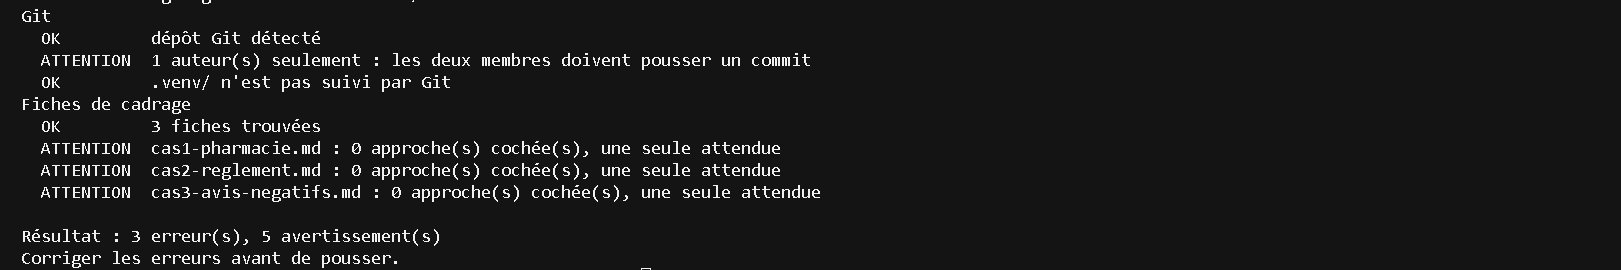
\includegraphics[width=0.88\textwidth]{avant.png}
\caption{Diagnostic initial avant correction.}
\end{figure}

\newpage

\section*{2. État après correction}

Après la complétion des fiches, le diagnostic reconnaît correctement une approche pour chacun des trois cas étudiés :

\begin{itemize}
    \item règles métier pour la vérification des ordonnances en pharmacie ;
    \item RAG pour les questions concernant le règlement intérieur ;
    \item machine learning pour la priorisation des avis négatifs.
\end{itemize}

Cette correction permet de faire disparaître les avertissements liés au cadrage. Le nombre d'erreurs passe ainsi de 3 à 2 et le nombre d'avertissements de 5 à 1.

Les deux erreurs encore affichées après correction concernent uniquement la vérification automatique de certaines dépendances présentes dans les \texttt{requirements}. Elles sont liées à l'installation ou à la détection des paquets par le script de diagnostic et ne remettent pas en cause le fonctionnement général du projet.

Les dépendances nécessaires ont bien été installées dans l'environnement de travail et l'installation s'est correctement déroulée. Ces deux messages correspondent donc à un problème de vérification de l'environnement par le diagnostic plutôt qu'à une erreur dans le développement ou dans le cadrage du projet.

Ils n'ont aucune incidence sur les choix réalisés dans les trois mini-cas ni sur la validation des principales étapes demandées dans le TP.

Le seul avertissement restant concerne le nombre d'auteurs de commits : un deuxième commit réalisé par l'autre membre du binôme permettra de compléter ce dernier point.

\begin{figure}[H]
\centering
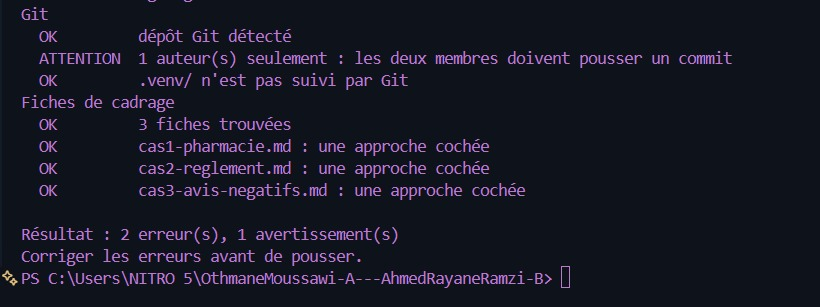
\includegraphics[width=0.88\textwidth]{Apres.jpeg}
\caption{Diagnostic après correction des fiches.}
\end{figure}

\section*{3. Comparaison et conclusion}

\begin{center}
\begin{tabular}{lcc}
\toprule
\textbf{Contrôle} & \textbf{Avant} & \textbf{Après} \\
\midrule
Approches cochées & 0 & 3 \\
Erreurs affichées & 3 & 2 \\
Avertissements & 5 & 1 \\
\bottomrule
\end{tabular}
\end{center}

La comparaison entre les deux diagnostics montre une amélioration nette du projet. Les trois décisions de cadrage sont désormais correctement renseignées et reconnues par le script de vérification. Le nombre d'avertissements passe également de cinq à un seul.

Les deux erreurs encore visibles dans le diagnostic final ne correspondent pas à des erreurs de conception ou de réalisation du TP. Elles sont uniquement liées au mécanisme de vérification automatique de l'installation de certaines dépendances Python. Les paquets nécessaires ont bien été installés et l'environnement de travail est fonctionnel.

Ces messages n'empêchent donc ni l'exécution du projet ni la poursuite des prochaines étapes. Le seul point organisationnel restant est la réalisation d'un commit personnel par le second membre du binôme.

Ce TP a ainsi permis de mettre en place une base de projet structurée, reproductible et versionnée, tout en définissant clairement les approches d'intelligence artificielle adaptées aux trois cas étudiés. Cette base pourra être réutilisée et enrichie durant les prochaines étapes du projet.

\end{document}